\documentclass[../../main.tex]{subfiles}
\begin{document}
\graphicspath{{figures/}{lectures/02_regularization/figures/}}
\section{Regularization}
\begin{frame}[plain]
  \vfill\begin{center}{\Huge \textcolor{blue}{Regularization}}\end{center}\vfill
\end{frame}
\begin{frame}{Polynomial Regression}

In 1D polynomial regression, we fit a model
$$ f_\theta(x) := \theta^\top \phi(x) = \sum_{j=0}^p \theta_j x^j $$
that is linear in $\theta$ but non-linear in $x$ because the features 
$$\phi(x) = [1\; x\; \ldots\; x^p]$$ 
are non-linear. Using these features, we can fit any polynomial of degree $p$.

\end{frame}


%%%%%%%%%%%%%%%%%%%%%%%%%%
\begin{frame}[fragile]{Polynomials Fit the Data Well}

Let's generate a synthetic dataset for this demonstration:

\begin{lstlisting}
from sklearn.pipeline import Pipeline
from sklearn.preprocessing import PolynomialFeatures
from sklearn.linear_model import LinearRegression

np.random.seed(0)
n_samples = 30
X = np.sort(np.random.rand(n_samples))
y = true_fn(X) + np.random.randn(n_samples) * 0.1

X_test = np.linspace(0, 1, 100)
plt.plot(X_test, true_fn(X_test), label="True function")
plt.scatter(X, y, edgecolor='b', s=20, label="Samples")

\end{lstlisting}



\end{frame}


%%%%%%%%%%%%%%%%%%%
\begin{frame}{Polynomials Fit the Data Well}

\begin{figure}[h]
    \centering
    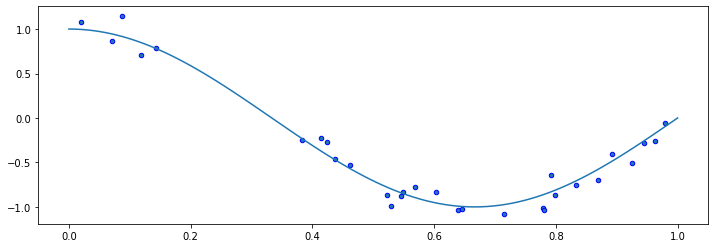
\includegraphics[width=1\textwidth]{output_1.png}  % Ajusta el nombre y la ruta de la imagen
\end{figure}

\end{frame}
%%%%%%%%%%%%%%%%%%%

\begin{frame}[fragile]{Polynomials Fit the Data Well}
Quadratic or cubic polynomials improve the fit of a linear model.

\begin{lstlisting}
degrees = [1, 2, 3]
plt.figure(figsize=(14, 5))
for i in range(len(degrees)):
    ax = plt.subplot(1, len(degrees), i + 1)

    polynomial_features = PolynomialFeatures(degree=degrees[i], include_bias=False)
    linear_regression = LinearRegression()
    pipeline = Pipeline([("pf", polynomial_features), ("lr", linear_regression)])
    pipeline.fit(X[:, np.newaxis], y)

    ax.plot(X_test, true_fn(X_test), label="True function")    
    ax.plot(X_test, pipeline.predict(X_test[:, np.newaxis]), label="Model")
    ax.scatter(X, y, edgecolor='b', s=20, label="Samples")
    ax.set_xlim((0, 1))
    ax.set_ylim((-2, 2))
    ax.legend(loc="best")
    ax.set_title("Polynomial of Degree {}".format(degrees[i]))
\end{lstlisting}

\end{frame}


%%%%%%%%%%%%%%%%%%%
\begin{frame}{Polynomials Fit the Data Well}

\begin{figure}[h]
    \centering
    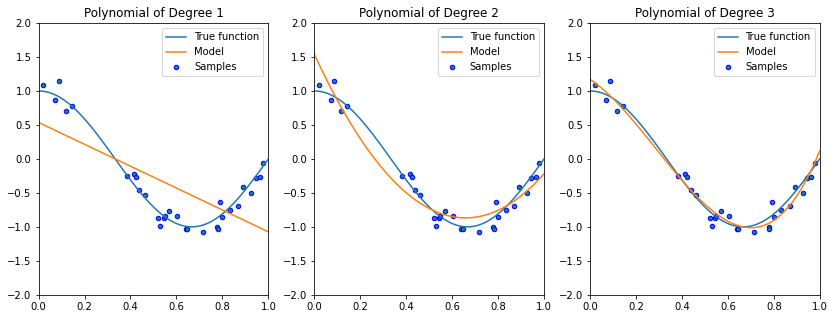
\includegraphics[width=1\textwidth]{output_2.png}  % Ajusta el nombre y la ruta de la imagen

\end{figure}

\end{frame}

%%%%%%%%%%%%%%%%%%%
\begin{frame}[fragile]{Towards Higher-Degree Polynomial Features?}
As we increase the complexity of our model class to include even higher degree polynomials, we are able to fit the data even better. What happens if we further increase the degree of the polynomial?
\begin{lstlisting}
degrees = [30]
plt.figure(figsize=(14, 5))
for i in range(len(degrees)):
    ax = plt.subplot(1, len(degrees), i + 1)

    polynomial_features = PolynomialFeatures(degree=degrees[i], include_bias=False)
    linear_regression = LinearRegression()
    pipeline = Pipeline([("pf", polynomial_features), ("lr", linear_regression)])
    pipeline.fit(X[:, np.newaxis], y)
    
    X_test = np.linspace(0, 1, 100)
    ax.plot(X_test, true_fn(X_test), label="True function")    
    ax.plot(X_test, pipeline.predict(X_test[:, np.newaxis]), label="Model")
\end{lstlisting}

\end{frame}
%%%%%%%%%%%%%%%%%%%
\begin{frame}[fragile]{Towards Higher-Degree Polynomial Features?}
\begin{lstlisting}[firstnumber=14]  % Comienza desde la línea 9
    ax.scatter(X, y, edgecolor='b', s=20, label="Samples")
    ax.set_xlim((0, 1))
    ax.set_ylim((-2, 2))
    ax.legend(loc="best")
    ax.set_title("Polynomial of Degree {}".format(degrees[i]))
\end{lstlisting}
%%%%%%%%%%%%%%%%%%%
\begin{figure}[h]
    \centering
    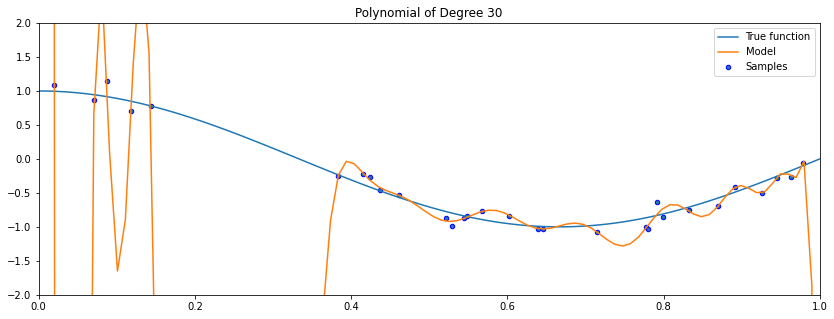
\includegraphics[width=0.85\textwidth]{output_3.png}  % Ajusta el nombre y la ruta de la imagen
\end{figure}

\end{frame}
%%%%%%%%%%%%%%%%%%%

\begin{frame}{Overfitting}

Overfitting is one of the most common failure modes of machine learning.
 \begin{itemize}
     \item A very expressive model (e.g., a high degree polynomial) fits the training dataset perfectly.
 \end{itemize}
 \begin{itemize}
     \item But the model makes highly incorrect predictions outside this dataset, and doesn't generalize.
 \end{itemize}

\vspace{0.5cm}
\textbf{How to Fix Overfitting} \\
We will see many ways of dealing with overfitting, but here are some ideas:


     \begin{itemize}
         \item Use a simpler model family (linear models vs. neural nets)
     \end{itemize}
 
     \begin{itemize}
         \item Keep the same model, but collect more training data 
     \end{itemize}

      \begin{itemize}
          \item Modify the training process to penalize overly complex models.
      \end{itemize}


 
\end{frame}
%%%%%%%%%%%%%%%%%%%
\begin{frame}{Underfitting}

A related failure mode is underfitting.
 \begin{itemize}
     \item A small model (e.g. a straight line), will not fit the training data well.
 \end{itemize}
 \begin{itemize}
     \item Therefore, it will also not be accurate on new data.
 \end{itemize} 

Finding the tradeoff between overfitting and underfitting is one of the main challenges in applying machine learning.

\vspace{0.5cm}
\textbf{How to Fix Underfitting} \\
What if our model doesn't fit the training set well? Try the following:

     \begin{itemize}
         \item Create richer features that will make the dataset easier to fit.
     \end{itemize}
 
     \begin{itemize}
         \item Use a more expressive model family (higher degree polynomials) 
     \end{itemize}

      \begin{itemize}
          \item Try to improve your optimization algorithm
      \end{itemize}


\end{frame}
%%%%%%%%%%%%%%%%%%%

\begin{frame}[fragile]{Overfitting vs. Underfitting: Evaluation}

We can diagnose overfitting and underfitting by measuring performance on a separate held out dataset (not used for training).

\begin{itemize}
    \item If training performance is high but holdout performance is low, we are overfitting.
\end{itemize}
\begin{itemize}
    \item If training performance is low and holdout performance is low, we are underfitting.
\end{itemize}


\begin{lstlisting}
degrees = [1, 20, 5]
titles = ['Underfitting', 'Overfitting', 'A Good Fit']
plt.figure(figsize=(14, 5))
for i in range(len(degrees)):
    ax = plt.subplot(1, len(degrees), i + 1)

    polynomial_features = PolynomialFeatures(degree=degrees[i], include_bias=False)
    linear_regression = LinearRegression()
    pipeline = Pipeline([("pf", polynomial_features), ("lr", linear_regression)])
    pipeline.fit(X[:, np.newaxis], y)
    ax.plot(X_test, true_fn(X_test), label="True function")
    ax.plot(X_test, pipeline.predict(X_test[:, np.newaxis]), label="Model")

\end{lstlisting}
\end{frame}
%%%%%%%%%%%%%%%%%%%
\begin{frame}[fragile]{Overfitting vs. Underfitting: Evaluation}


\begin{lstlisting}[firstnumber=13]
    ax.plot(X_test, pipeline.predict(X_test[:, np.newaxis]), label="Model")
    ax.scatter(X, y, edgecolor='b', s=20, label="Samples", alpha=0.2)
    ax.scatter(X_holdout[::3], y_holdout[::3], edgecolor='r', s=20, label="Samples")
    ax.set_xlim((0, 1))
    ax.set_ylim((-2, 2))
    ax.legend(loc="best")
    ax.set_title("{} (Degree {})".format(titles[i], degrees[i]))
    ax.text(0.05,-1.7, 'Holdout MSE: %.4f' % ((y_holdout-pipeline.predict(X_holdout[:, np.newaxis]))**2).mean())
\end{lstlisting}
\end{frame}


%%%%%%%%%%%%%%%%%%%
\begin{frame}[fragile]{Overfitting vs. Underfitting: Evaluation}

\begin{figure}[h]
    \centering
    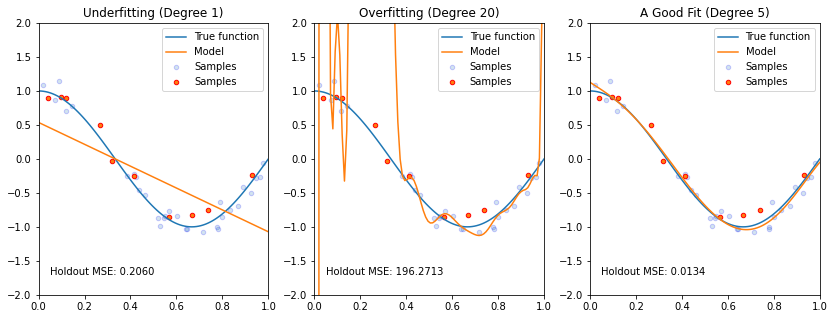
\includegraphics[width=0.95\textwidth]{output_4.png}  % Ajusta el nombre y la ruta de la imagen
\end{figure}

\end{frame}
%%%%%%%%%%%%%%%%%%%

 \begin{frame}[fragile]{Regularization (definition)}

The idea of regularization is to train models with an augmented objective $J : \mathcal{M} \to \mathbb{R}$ defined over a training dataset $\mathcal{D}$ of size $n$ as

$$J(f) = \underbrace{\frac{1}{n} \sum_{i=1}^n L(y^{(i)}, f(x^{(i)}))}_\text{Learning Objective} + \underbrace{\lambda \cdot R(f)}_\text{New Regularization Term}$$

\begin{itemize}
    \item The regularizer $R : \mathcal{M} \to \mathbb{R}$ penalizes models that are complex. 
\end{itemize}
\begin{itemize}
    \item The hyperparameter $\lambda > 0$ controls the strength of the regularizer. 
\end{itemize}



\end{frame}
%%%%%%%%%%%%%%%%%%%

 \begin{frame}[fragile]{Regularization (definition)}
Let's dissect the components of this objective:

$$J(f) = \frac{1}{n} \sum_{i=1}^n L(y^{(i)}, f(x^{(i)})) + \lambda \cdot R(f).$$

\begin{itemize}
    \item A loss function $L(y, f(x))$ such as the mean squared error. 
\end{itemize}

\begin{itemize}
    \item A regularizer $R : \mathcal{M} \to \mathbb{R}$ that penalizes models that are overly complex.
\end{itemize}

\begin{itemize}
    \item A regularization parameter $\lambda > 0$, which controls the strength of the regularizer.
\end{itemize}

When the model $f_\theta$ is parametrized by parameters $\theta$, we also use the following notation:

$$J(\theta) = \frac{1}{n} \sum_{i=1}^n L(y^{(i)}, f_\theta(x^{(i)})) + \lambda \cdot R(\theta).$$
\end{frame}
%%%%%%%%%%%%%%%%%%%
\begin{frame}[fragile]{L2 Regularization: Definition (Ridge Regression)}
 
How can we define a regularizer $R: \mathcal{M} \to \mathbb{R}$ to control the complexity of a model $f \in \mathcal{M}$?


In the context of linear models $f_\theta(x) = \theta^\top x$, a widely used approach is L2 regularization, which defines the following objective:
$$J(\theta) = \frac{1}{n} \sum_{i=1}^n L(y^{(i)}, \theta^\top x^{(i)}) + \frac{\lambda}{2} \cdot ||\theta||_2^2.$$

\begin{itemize}
    \item The regularizer $R : \Theta \to \mathbb{R}$ is the function $R(\theta) = ||\theta||_2^2 = \sum_{j=1}^d \theta_j^2.$ This is also known as the L2 norm of $\theta$.
\end{itemize}

\begin{itemize}
    \item The regularizer penalizes large parameters. This prevents us from relying on any single feature and penalizes very irregular solutions.
\end{itemize}

\begin{itemize}
    \item L2 regularization can be used with most models (linear, neural, etc.)
\end{itemize}

\end{frame}
%%%%%%%%%%%%%%%%%%%
\begin{frame}[fragile]{L2 Regularization for Polynomial Regression}

Let's consider an application to the polynomial model we have seen so far. Given polynomial features $\phi(x)$, we optimize the following objective:

$$ J(\theta) = \frac{1}{2n} \sum_{i=1}^n \left( y^{(i)} - \theta^\top \phi(x^{(i)}) \right)^2 + \frac{\lambda}{2} \cdot ||\theta||_2^2. $$

We implement regularized and polynomial regression of degree 15 on three random training sets sampled from the same distribution:


\begin{lstlisting}
from sklearn.linear_model import Ridge
degrees = [15, 15, 15]
plt.figure(figsize=(14, 5))
for idx, i in enumerate(range(len(degrees))):
    # sample a dataset
    np.random.seed(idx)
    n_samples = 30
    X = np.sort(np.random.rand(n_samples))
    y = true_fn(X) + np.random.randn(n_samples) * 0.1
\end{lstlisting}
\end{frame}

\begin{frame}[fragile]{L2 Regularization for Polynomial Regression}
\begin{lstlisting}[firstnumber=11]
    # fit a least squares model
    polynomial_features = PolynomialFeatures(degree=degrees[i], include_bias=False)
    linear_regression = LinearRegression()
    pipeline = Pipeline([("pf", polynomial_features), ("lr", linear_regression)])
    pipeline.fit(X[:, np.newaxis], y)
    # fit a Ridge model
    polynomial_features = PolynomialFeatures(degree=degrees[i], include_bias=False)
    linear_regression = Ridge(alpha=0.1) # sklearn uses alpha instead of lambda
    pipeline2 = Pipeline([("pf", polynomial_features), ("lr", linear_regression)])
    pipeline2.fit(X[:, np.newaxis], y) 
    # visualize results
    ax = plt.subplot(1, len(degrees), i + 1)
\end{lstlisting}
\end{frame}

\begin{frame}[fragile]{L2 Regularization for Polynomial Regression}
\begin{lstlisting}[firstnumber=22]
    # ax.plot(X_test, true_fn(X_test), label="True function")    
    ax.plot(X_test, pipeline.predict(X_test[:, np.newaxis]), label="No Regularization")
    ax.plot(X_test, pipeline2.predict(X_test[:, np.newaxis]), label="L2 Regularization")    
    ax.scatter(X, y, edgecolor='b', s=20, label="Samples")
    ax.set_xlim((0, 1))
    ax.set_ylim((-2, 2))
    ax.legend(loc="best")
    ax.set_title("Dataset sample #{}".format(idx))
\end{lstlisting}
\end{frame}


\begin{frame}[fragile]{L2 Regularization for Polynomial Regression}
\begin{figure}[h]
    \centering
    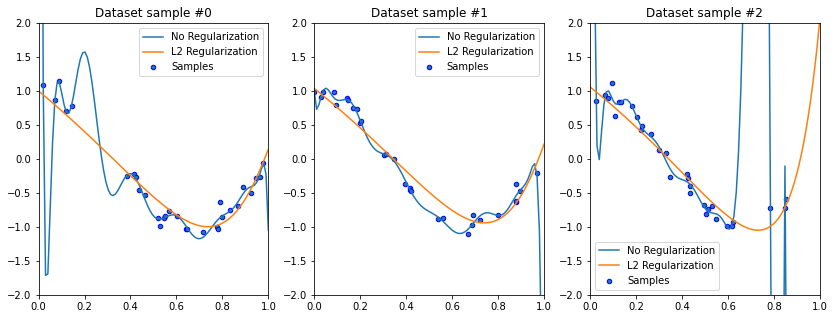
\includegraphics[width=0.95\textwidth]{output_5.png}  % Ajusta el nombre y la ruta de la imagen
\end{figure}
\end{frame}

%%%%%%%%%%%%%%%%%%%%%%%%%%%%%%%%%%%%%%%%%%%
\begin{frame}[fragile]{L2 Regularization for Polynomial Regression}


In order to define a very irregular function, we need very large polynomial weights.
Forcing the model to use small weights prevents it from learning irregular functions.

\vspace{0.5cm}
\begin{lstlisting}
print('Non-regularized weights of the polynomial model need to be large to fit every point:')
print(pipeline.named_steps['lr'].coef_[:4])
print()

print('By regularizing the weights to be small, we force the curve to be more regular:')
print(pipeline2.named_steps['lr'].coef_[:4])
\end{lstlisting}
\end{frame}
%%%%%%%%%%%%%%%%%%%%%%%%%%%%%%%%%%%%%%%%%%%

\begin{frame}[fragile]{Normal Equations for Regularized Models}

Let $L(\theta) = \frac{1}{2} (X \theta - y)^\top  (X \theta - y)$ be our least squares objective. We can write the L2-regularized objective as:
$$ J(\theta) = \frac{1}{2} (X \theta - y)^\top  (X \theta - y) + \frac{1}{2} \lambda ||\theta||_2^2 $$

This allows us to derive the gradient as follows:
\begin{align*}
\nabla_\theta J(\theta) 
& = \nabla_\theta \left( \frac{1}{2} (X \theta - y)^\top  (X \theta - y) + \frac{1}{2} \lambda ||\theta||_2^2 \right) \\
& = \nabla_\theta \left( L(\theta) + \frac{1}{2} \lambda \theta^\top \theta \right) \\
& = \nabla_\theta L(\theta) + \lambda \theta \\
& = (X^\top X) \theta - X^\top y + \lambda \theta \\
& = (X^\top X + \lambda I) \theta - X^\top y
\end{align*}

We used the derivation of the normal equations for least squares to obtain $\nabla_\theta L(\theta)$ as well as the fact that: $\nabla_x x^\top x = 2 x$.
\end{frame}
%%%%%%%%%%%%%%%%%%%%%%%%%%%%%%%%%%%%%%%%%%%


\begin{frame}[fragile]{Normal Equations for Regularized Models}

We can set the gradient to zero to obtain normal equations for the Ridge model:
$$ (X^\top X + \lambda I) \theta = X^\top y. $$

Hence, the value $\theta^*$ that minimizes this objective is given by:
$$ \theta^* = (X^\top X + \lambda I)^{-1} X^\top y.$$

Note that the matrix $(X^\top X + \lambda I)$ is always invertible, which addresses a problem with least squares that we saw earlier.


\end{frame}


%%%%%%%%%%%%%%%%%%%%%%%%%%%%%%%%%%%%%%%%%%%

\begin{frame}[fragile]{L1 Regularization: Definition (Lasso Regression)}

The idea of regularization is to train models with an augmented objective $J : \mathcal{M} \to \mathbb{R}$ defined over a training dataset $\mathcal{D}$ of size $n$ as
$$ J(f) = \frac{1}{n} \sum_{i=1}^n L(y^{(i)}, f(x^{(i)})) + \lambda \cdot R(f). $$

\begin{itemize}
    \item A loss function $L(y, f(x))$ such as the mean squared error.
\end{itemize}

\begin{itemize}
    \item A regularizer $R : \mathcal{M} \to \mathbb{R}$ that penalizes models that are overly complex.
\end{itemize}

Another closely related approach to regularization is to penalize the size of the weights using the L1 norm. 
\end{frame}
%%%%%%%%%%%%%%%%%%%%%%%%%%%%%%%%%%%%%%%%%%%
\begin{frame}[fragile]{L1 Regularization: Definition (Lasso Regression)}


In the context of linear models $f(x) = \theta^\top x$, L1 regularization yields the following objective:
$$ J(\theta) = \frac{1}{n} \sum_{i=1}^n L(y^{(i)}, \theta^\top x^{(i)}) + \lambda \cdot ||\theta||_1. $$

\begin{itemize}
    \item The regularizer $R : \mathcal{M} \to \mathbb{R}$ is $R(\theta) = ||\theta||_1 = \sum_{j=1}^d |\theta_j|.$ This is known as the L1 norm of $\theta$.
\end{itemize}


\begin{itemize}
    \item This regularizer also penalizes large weights. It additionally forces most weights to decay to zero, as opposed to just being small.
\end{itemize}


\end{frame} 
%%%%%%%%%%%%%%%%%%%%%%%%%%%%%%%%%%%%%%%%%%%
\begin{frame}[fragile]{Sparsity: Definition}
A vector is said to be sparse if a large fraction of its entries is zero.
\vspace{0.5cm}
L1-regularized linear regression produces \textit{sparse parameters} $\theta$.
 \begin{itemize}
     \item This is makes the model more interpretable
 \end{itemize}
\begin{itemize}
    \item It also makes it computationally more tractable in very large dimensions.
\end{itemize}

\end{frame}
%%%%%%%%%%%%%%%%%%%%%%%%%%%%%%%%%%%%%%%%%%%
\begin{frame}[fragile]{Sparsity: Ridge Model}

To better understand sparsity, we fit Ridge and Lasso on the UCI diabetes dataset and observe the magnitude of each weight (colored lines) as a function of the regularization parameter.



\begin{lstlisting}
from sklearn.datasets import load_diabetes
from sklearn.linear_model import Ridge
from matplotlib import pyplot as plt

X, y = load_diabetes(return_X_y=True)

# create ridge coefficients
alphas = np.logspace(-5, 2,  )
ridge_coefs = []
for a in alphas:
    ridge = Ridge(alpha=a, fit_intercept=False)
    ridge.fit(X, y)
    ridge_coefs.append(ridge.coef_)
# plot ridge coefficients
plt.figure(figsize=(14, 5))
plt.plot(alphas, ridge_coefs)
\end{lstlisting}
\end{frame}
%%%%%%%%%%%%%%%%%%%%%%%%%%%%%%%%%%%%%%%%%%%

\begin{frame}[fragile]{Sparsity: Ridge Model}
\begin{lstlisting}[firstnumber=17]
plt.xscale('log')
plt.xlabel('Regularization parameter (lambda)')
plt.ylabel('Magnitude of model parameters')
plt.title('Ridge coefficients as a function of the regularization')
plt.axis('tight')
\end{lstlisting}

\begin{figure}[h]
    \centering
    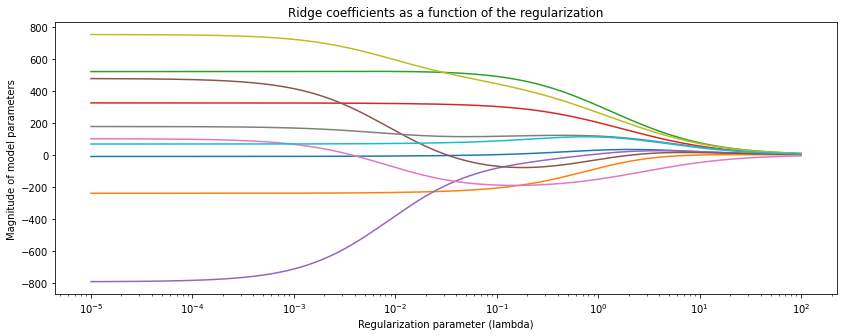
\includegraphics[width=0.85\textwidth]{output_6.png}  % Ajusta el nombre y la ruta de la imagen
\end{figure}
\end{frame}


\begin{frame}[fragile]{Sparsity: Ridge vs. Lasso}
The Lasso parameters become progressively smaller, until they reach exactly zero, and then they stay at zero.

\begin{lstlisting}
import warnings
warnings.filterwarnings("ignore")
from sklearn.datasets import load_diabetes
from sklearn.linear_model import lars_path

# create lasso coefficients    
X, y = load_diabetes(return_X_y=True)
_, _, lasso_coefs = lars_path(X, y, method='lasso')
xx = np.sum(np.abs(lasso_coefs.T), axis=1)
# plot ridge coefficients
plt.figure(figsize=(14, 5))
plt.subplot('121')    
plt.plot(alphas, ridge_coefs)
plt.xscale('log')
plt.xlabel('Regularization Strength (lambda)')
plt.ylabel('Magnitude of model parameters')

\end{lstlisting}
\end{frame}


\begin{frame}[fragile]{Sparsity: Ridge vs. Lasso}
\begin{lstlisting}[firstnumber=17]
plt.title('Ridge coefficients as a function of regularization strength $\lambda$')
plt.axis('tight')
# plot lasso coefficients
plt.subplot('122') 
plt.plot(3500-xx, lasso_coefs.T)
ymin, ymax = plt.ylim()
plt.ylabel('Magnitude of model parameters')
plt.xlabel('Regularization Strength (lambda)')
plt.title('LASSO coefficients as a function of regularization strength $\lambda$')
plt.axis('tight')
\end{lstlisting}
\end{frame}
\begin{frame}[fragile]{Sparsity: Ridge vs. Lasso}
\begin{figure}[h]
    \centering
    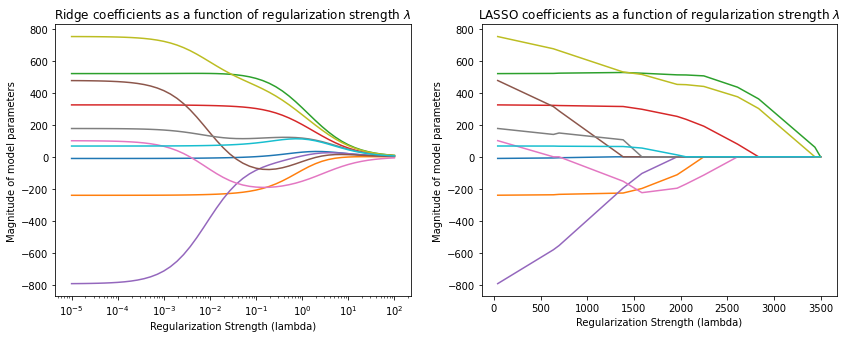
\includegraphics[width=0.95\textwidth]{output_7.png}  % Ajusta el nombre y la ruta de la imagen
\end{figure}
\end{frame}



\begin{frame}[fragile]{Regularizing via Constraints}

Consider a regularized problem with a penalty term:
$$ \min_{\theta \in \Theta} L(\theta) + \lambda \cdot R(\theta). $$

Alternatively, we may enforce an explicit constraint on the complexity of the model:
\begin{align*}
\min_{\theta \in \Theta} \; & L(\theta) \\
\text{such that } \; & R(\theta) \leq \lambda'
\end{align*}

We will not prove this, but solving this problem is equivalent to solving the penalized problem for some $\lambda > 0$ that's different from $\lambda'$.

In other words, 
\begin{itemize}
    \item We can regularize by explicitly enforcing $R(\theta)$ to be less than a value instead of penalizing it.
\end{itemize}
\begin{itemize}
    \item For each value of $\lambda$, we are implicitly setting a constraint of $R(\theta)$.
\end{itemize}
\end{frame}

\begin{frame}[fragile]{Regularizing via Constraints: Example}

This is what constraint-based regularization looks like for the linear models we have seen thus far:
\begin{align*}
\min_{\theta \in \Theta} \; & \frac{1}{2n} \sum_{i=1}^n \left( y^{(i)} - \theta^\top x^{(i)} \right)^2 \\
\text{such that } \; & ||\theta|| \leq \lambda'
\end{align*}

where $||\cdot||$ can either be the L1 or L2 norm.

\end{frame}


\begin{frame}[fragile]{L1 vs. L2 Regularization}

The following image by Divakar Kapil and Hastie et al. explains the difference between the two norms.

\begin{figure}[h]
    \centering
    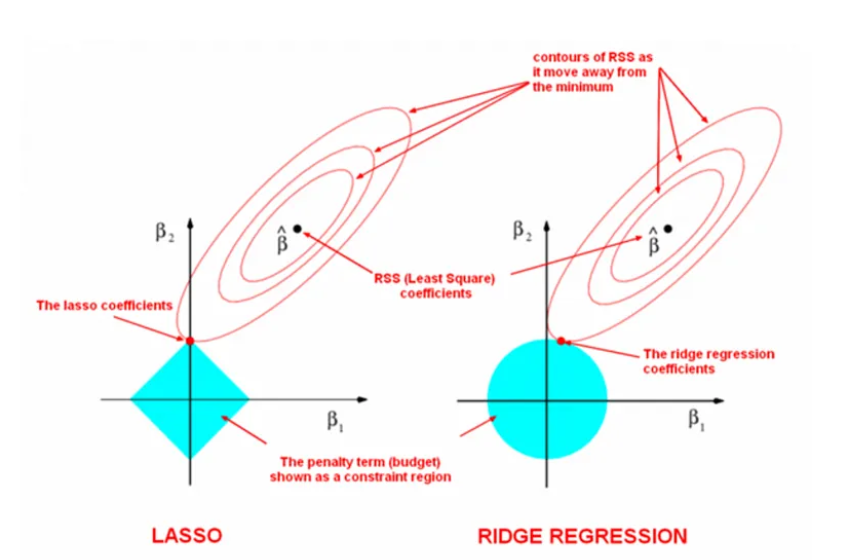
\includegraphics[width=0.65\textwidth]{image1.png}  % Ajusta el nombre y la ruta de la imagen
\end{figure}
\end{frame}

\begin{frame}[fragile]{A Framework for Applying Supervised Learning}

\textbf{Why Do We Need A Framework for Applying Machine Learning?}

It helps to be principled. Consider the following questions:
 \begin{itemize}
     \item How do we detect overfitting or underfitting?
     \item How to tune the degree $p$ in polynomial regression?
     \item How do we know that our model is ready to be deployed?
 \end{itemize}

Our framework will provide answers that yield good models.
\vspace{0.5cm}

\textbf{What Is A Good Supervised Learning Model?}
A good predictive model is one that makes \textbf{accurate predictions} on \textbf{new data} that it has not seen at training time.

\begin{itemize}
    \item Accurate object detection in new scenes
    \item Correct translation of new sentences
\end{itemize}


\end{frame}
\begin{frame}[fragile]{A Framework for Applying Supervised Learning}
\textbf{Datasets for Model Development}

When developing machine learning models, the first step is to usually split the data into three sets:

\begin{itemize}
    \item \textbf{Training set:} Data on which we train our algorithms.
    \item \textbf{Development set (validation or holdout set):} Data used for tuning algorithms.
    \item \textbf{Test set:} Data used to evaluate the final performance of the model.
\end{itemize}
\vspace{0.5cm}

\textbf{Model Development Workflow}
The typical way in which these datasets are used is:

\begin{enumerate}
    \item \textbf{Training:} Try a new model and fit it on the training set. 
    \item \textbf{Model Selection:} Estimate performance on the development set using metrics. Based on results, try a new model idea in step \#1.
    \item \textbf{Evaluation}: Finally, estimate real-world performance on test set.
\end{enumerate}

\end{frame}

\begin{frame}[fragile]{A Framework for Applying Supervised Learning}

\textbf{How to Use Validation Set}
There are many ways to tune a model at step \#2:
\begin{itemize}
    \item Increase/decrease degree of polynomial based on over/underfitting.
    \item Perform grid search to find best hyper-parameter \textbf{\textit{p}}.
    \item Understand which features to add to the model.
\end{itemize}

\vspace{0.5cm}

\textbf{Validation and Test Sets}
These holdout sets are used to estimate real-world performance. How should one choose the development and test set?

\begin{itemize}
    \item \textbf{Distributional Consistency:} The development and test sets should be from the data distribution we will see in production.
    \item \textbf{Dataset Size:} Should be large enough to estimate future performance: 30\% of the data on small tasks, ususally up to not more than a few thousand instances.
\end{itemize}
\end{frame}



\begin{frame}[fragile]{Cross-Validation}

If we don't have enough data for a validation set, we can do $K$-fold cross-validation.

We group the data into $K$ disjoint folds. We train the model $K$ times, each time using a different fold for testing, and the rest for training.

\begin{figure}[h]
    \centering
    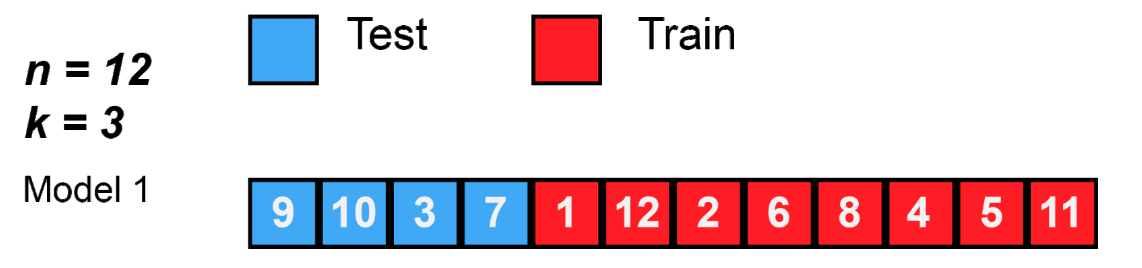
\includegraphics[width=0.8\textwidth]{image_2.png}  % Ajusta el nombre y la ruta de la imagen
\end{figure}
\end{frame}

\begin{frame}[fragile]{Evaluating Supervised Learning Models}

\textbf{Data Distribution}

It is standard to assume that data is sampled from a probability distribution $\mathbb{P}$, which we will call the \textbf{data distribution}. We  denote this as

$$x, y \sim \mathbb{P} \;\;\;\text{ or }\;\;\; \mathcal{D} \sim \mathbb{P}.$$

The training set $\mathcal{D} = \{(x^{(i)}, y^{(i)}) \mid i = 1,2,...,n\}$ consists of \textit{independent and identically distributed (IID)} samples from $\mathbb{P}$.

\vspace{0.5cm}
\textbf{Data Distribution: IID Sampling}

The key assumption is that the training examples are \textit{independent and identically distributed (IID)}. 
\begin{itemize}
    \item Each training example is from the same distribution.
    \item This distribution doesn't depend on previous training examples.
\end{itemize}

\end{frame}


\begin{frame}[fragile]{Data Distribution: Example}

Let's implement an example of a data distribution in numpy.

\begin{lstlisting}
import numpy as np
np.random.seed(0)

def true_fn(X):
    return np.cos(1.5 * np.pi * X)
\end{lstlisting}

Let's visualize it.

\begin{lstlisting}
import matplotlib.pyplot as plt
plt.rcParams['figure.figsize'] = [12, 4]

X_test = np.linspace(0, 1, 100)
plt.plot(X_test, true_fn(X_test), label="True function")
plt.legend()
\end{lstlisting}
\end{frame}

\begin{frame}[fragile]{Data Distribution: Example}
\begin{figure}[h]
    \centering
    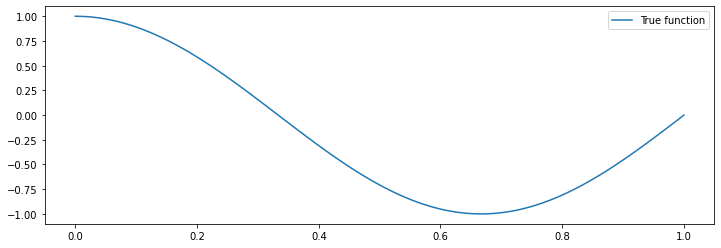
\includegraphics[width=1\textwidth]{output_8.png}  % Ajusta el nombre y la ruta de la imagen
\end{figure}
\end{frame}

\begin{frame}[fragile]{Data Distribution: Example}

Let's now draw samples from the distribution. We will generate random $x$, and then generate random $y$ using
$$ y = f(x) + \epsilon $$
for a random noise variable $\epsilon$.

\begin{lstlisting}
n_samples = 30

X = np.sort(np.random.rand(n_samples))
y = true_fn(X) + np.random.randn(n_samples) * 0.1
\end{lstlisting}

We can visualize the samples.

\begin{lstlisting}
plt.plot(X_test, true_fn(X_test), label="True function")
plt.scatter(X, y, edgecolor='b', s=20, label="Samples")
plt.legend()
\end{lstlisting}


\end{frame}

\begin{frame}[fragile]{Data Distribution: Example}

\begin{figure}[h]
    \centering
    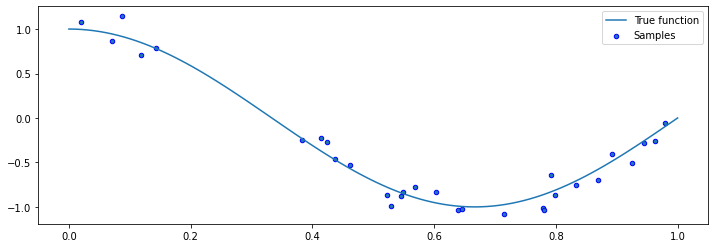
\includegraphics[width=1\textwidth]{output_9.png}  % Ajusta el nombre y la ruta de la imagen
\end{figure}
\end{frame}


\begin{frame}[fragile]{Holdout Dataset}
A holdout set 

$$\dot{\mathcal{D}} = \{(\dot{x}^{(i)}, \dot{y}^{(i)}) \mid i = 1,2,...,m\}$$

is sampled IID from the same distribution $\mathbb{P}$, and is distinct from the training dataset $\mathcal{D}$.

Let's generate a holdout dataset for the example we saw earlier.

\begin{lstlisting}
n_samples, n_holdout_samples = 30, 30

X = np.sort(np.random.rand(n_samples))
y = true_fn(X) + np.random.randn(n_samples) * 0.1
X_holdout = np.sort(np.random.rand(n_holdout_samples))
y_holdout = true_fn(X_holdout) + np.random.randn(n_holdout_samples) * 0.1

plt.plot(X_test, true_fn(X_test), label="True function")
plt.scatter(X, y, edgecolor='b', s=20, label="Samples")
plt.scatter(X_holdout, y_holdout, edgecolor='r', s=20, label="Holdout Samples")
plt.legend()
\end{lstlisting}

\end{frame}

\begin{frame}[fragile]{Holdout Dataset}

\begin{figure}[h]
    \centering
    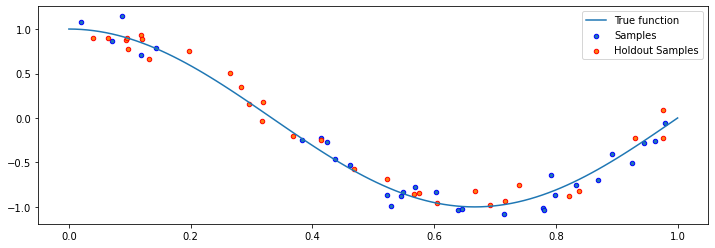
\includegraphics[width=1\textwidth]{output_10.png}  % Ajusta el nombre y la ruta de la imagen
\end{figure}
\end{frame}
\begin{frame}[fragile]{Performance on a Holdout Set}

Intuitively, a supervised model $f_\theta$ is "good" if it performs well on a holdout set $\dot{\mathcal{D}}$ according to some measure

$$
\frac{1}{m} \sum_{i=1}^m L\left(\dot y^{(i)}, f_\theta(\dot x^{(i)}) \right).
$$

Here, $L : \mathcal{X}\times\mathcal{Y} \to \mathbb{R}$ is a performance metric or a loss function that we get to choose.

The choice of the performance metric $L$ depends on the specific problem and our goals:

\begin{itemize}
    \item In classification, $L$ is often just accuracy: is $\dot y^{(i)} = f_\theta(\dot x^{(i)})$?
    \item $L$ can also implement other metrics: $R^2$ metric (see Homework 1) for regression, F1 score for document retrieval, etc.
\end{itemize}
\end{frame}

\begin{frame}[fragile]{Performance on a Holdout Set}

For example, in a classification setting, we may be interested in the accuracy of the model. Thus, we want the % of misclassified inputs
$$
\frac{1}{m} \sum_{i=1}^m \mathbb{I}\left(\dot y^{(i)} \neq f_\theta(\dot x^{(i)}) \right)
$$
to be small. 


Here $\mathbb{I}\left( A \right)$ is an \textbf{indicator} function that equals one if $A$ is true and zero otherwise.


For large enough holdout sets $\dot{\mathcal{D}}$, we will be estimating performance on new data from $\mathbb{P}$.

\vspace{0.4cm}
\textbf{When Does Supervised Learning Work?} 

\begin{itemize}
    \item For large enough training sets $\mathcal{D} \sim \mathbb{P}$, most models will \textit{generalize} to new data from $\mathbb{P}$. We should see the same performance on $\mathcal{D}$ and $\dot{\mathcal{D}} \sim \mathbb{P}$.
    \item When $\mathcal{D}$ is small, models may overfit $\mathcal{D}$ and perform poorly on new data from $\mathbb{P}$. We can detect this by evaluating them on $\dot{\mathcal{D}}$.
\end{itemize}
\end{frame}

\begin{frame}[fragile]{Why Does Supervised Learning Work?}

We have seen a number of supervised learning algorithms. Next, let's look more precisely at why they work (and why sometimes they don't).

\vspace{0.5cm}

\textbf{Recall: Supervised Learning}

Recall our intuitive definition of supervised learning.

\begin{figure}[h]
    \centering
    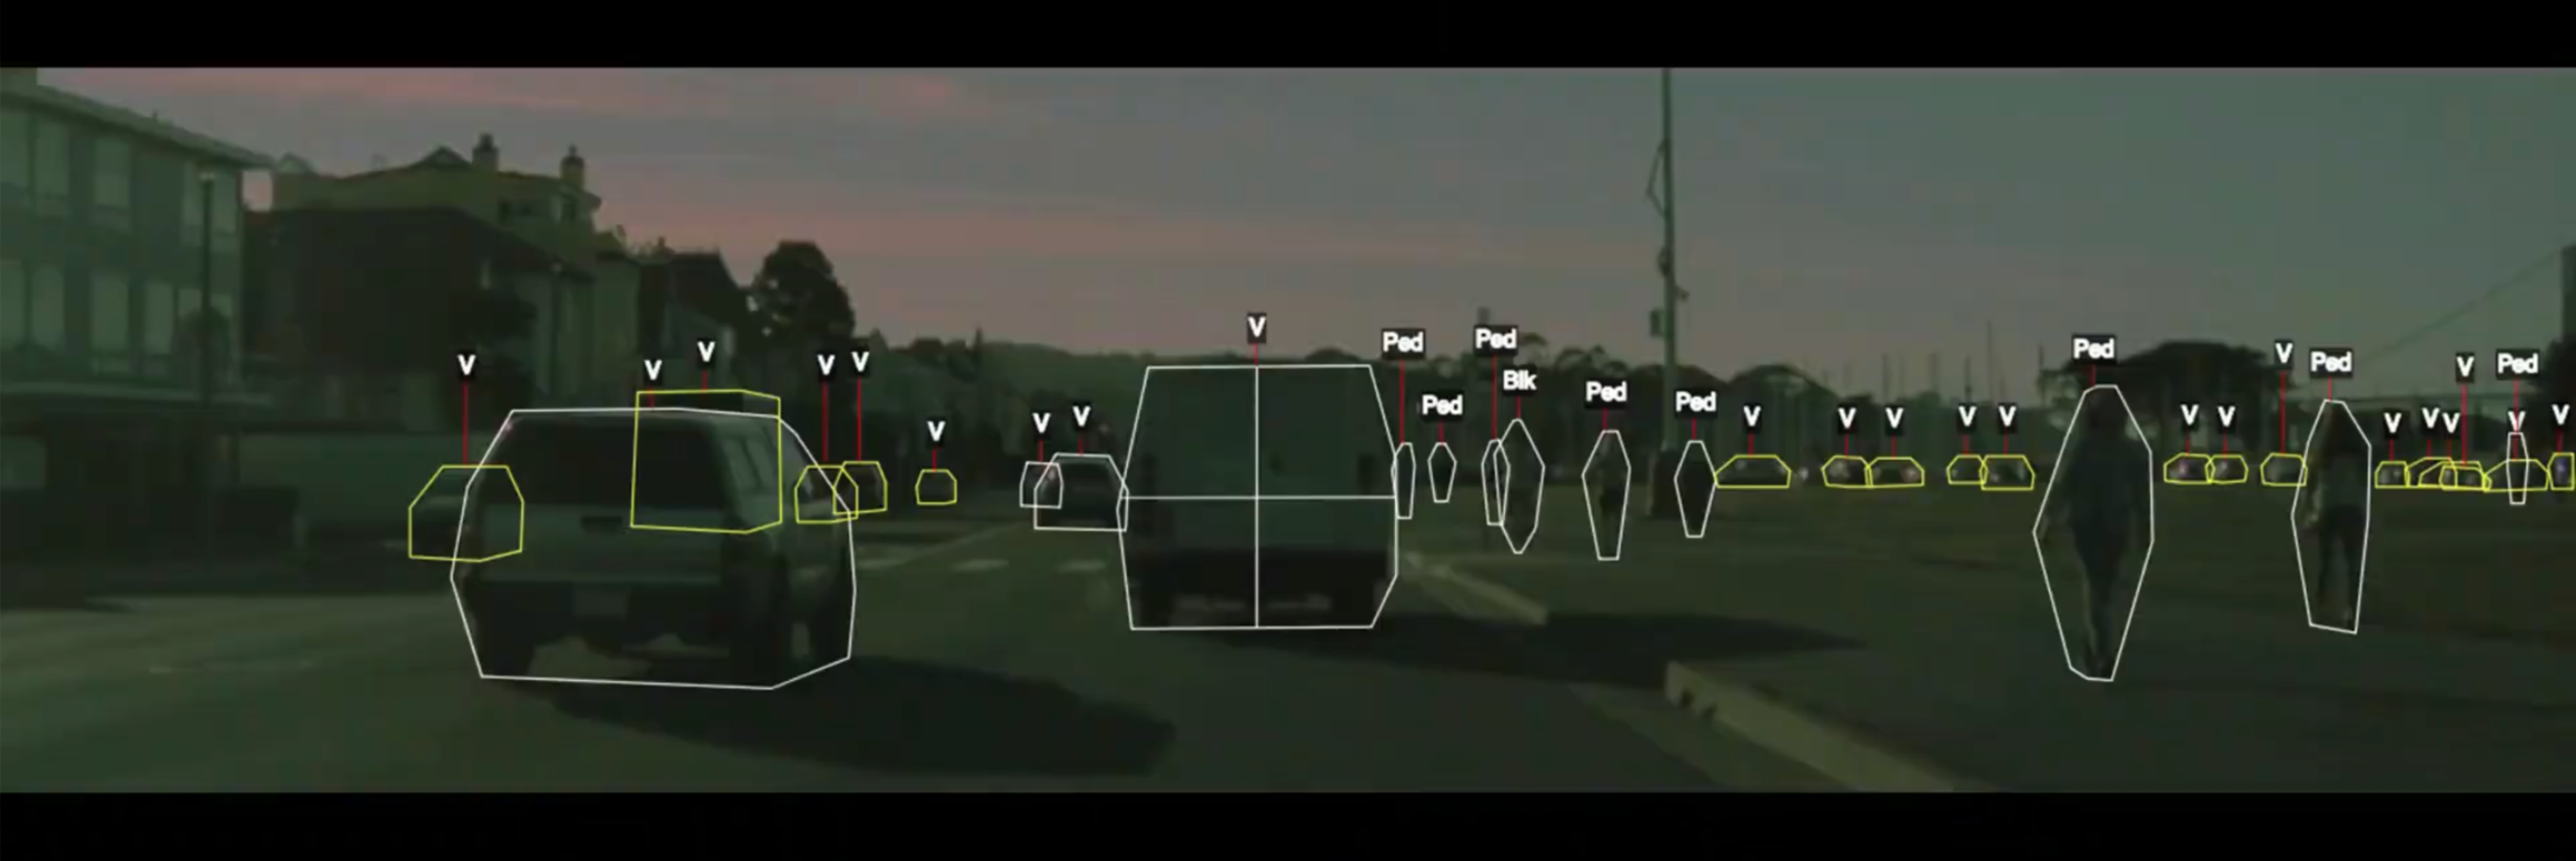
\includegraphics[width=0.65\textwidth]{tesla_data.png}  % Ajusta el nombre y la ruta de la imagen
\end{figure}


\begin{enumerate}
    \item First, we collect a dataset of labeled training examples.
    \item We train a model to output accurate predictions on this dataset.
\end{enumerate}
\end{frame}

\begin{frame}[fragile]{What Is A Good Supervised Learning Model?}

A good predictive model is one that makes \textbf{accurate predictions} on \textbf{new data} that it has not seen at training time.

\begin{itemize}
    \item Accurate object detection in new scenes
    \item Correct translation of new sentences
\end{itemize}

\vspace{0.5cm}

\textbf{Recall: Data Distribution}

We will assume that data is sampled from a probability distribution $\mathbb{P}$, which we will call the \textit{data distribution}. We will denote this as
$$x, y \sim \mathbb{P}.$$

The training set $\mathcal{D} = \{(x^{(i)}, y^{(i)}) \mid i = 1,2,...,n\}$ consists of \textit{independent and identically distributed (IID)} samples from $\mathbb{P}$.



\end{frame}
\end{document}
